\documentclass[i3]{oss}
\usepackage[english]{babel}
\usepackage{graphicx}

\usepackage{fullpage}
\usepackage{color}
\usepackage{soul}
%\usepackage{gensymb}
\usepackage{caption}
\usepackage{subcaption}
\usepackage[section]{placeins}
\usepackage{titlesec}
\usepackage{wrapfig}
\usepackage{color}
% Automatically introduces paragraph spacing
\usepackage{parskip}

% Lets Latex correctly interpret the symbols: < >
\usepackage[T1]{fontenc}

\setcounter{secnumdepth}{4}
\titleformat{\paragraph}
{\normalfont\normalsize\bfseries}{\theparagraph}{1em}{}
\titlespacing*{\paragraph}
{0pt}{3.25ex plus 1ex minus .2ex}{1.5ex plus .2ex}

\newcommand{\class}[1]{\texttt{#1}}
\newcommand{\method}[1]{\texttt{#1}}
\newcommand{\junit}{\emph{JUnit }}
\newcommand{\Daemon}{\class{Daemon  }}
\newcommand{\gloss}[1]{\textbf{#1}}
\newcommand{\col}[1]{\textcolor{red}{#1}}
\newcommand{\comment}[1]{{\huge \textcolor{green}{#1}}\\}

\begin{document}

\members{Joren Verspeurt {\small \texttt{(r0258417)} } \\ %# Commentaar
         Sophie Marien {\small \texttt{(s0216517)}}\\
         Stef Noten {\small \texttt{(s0211264)}}\\
         Toon Nolten {\small \texttt{(r0258654)}} \\
         Begeleider: Mario H. C. T.} % teamleden

\maketitlepage
\newpage
\tableofcontents
\pagebreak



%------------------------------------------------------ %
%														%
%           Introduction
%														%
%------------------------------------------------------ %
\section*{Introduction}
\label{ssec:introduction}
%introductie en de belangrijkste elementen van ons ontwerp
In the first iteration we assessed the design and implementation of \junit and in the second iteration we extended it with a daemon that would continuously test a given project according to a policy chosen by the user.
In this iteration we have to expand \junit to allow a combination of multiple policies. The combination of policies has to be fair. After the expansion we have to refactor the whole project and analyse it like we did in iteration 1.

In sections \ref{ss:designext} and \ref{ss:implemenext}, the implementation of the composition of policies is discussed and the design of this extension is explained.
In sections \ref{ss:refactoring} and \ref{ss:analyse} the refactoring and the analysis of our extension of \junit are discussed. 
In the final section we discuss and evaluate the project.


%------------------------------------------------------ %
%														%
%           Activity 1
%														%
%------------------------------------------------------ %
\section{Activity 1: extension}

\subsection{Policies: current design}
\label{ss:current-design}

In the current design, policies are represented by the \class{IPolicy} interface.
This interface exposes the method \method{apply}, which transforms a \junit \class{Request} into a \class{Request} that complies with the properties of the policy.
In the previous assignment, all the specified policies are sorting policies.
The root class for all sorting policies is the \class{SortingPolicy} class. It's \method{apply} method thus transforms a given \class{Request} into a \class{Request} that is sorted according to the policy's rules.

\comment{diagrammen}

%------------------------------------------------------ %
%---------------------------------------------------
%           Design
% ---------------------------------------------------
%------------------------------------------------------ %
\subsection{Design}
\label{ss:designext}

It should be possible to combine sorting policies into a new sorting policy.
These combined policies should be treated in the same way as other policies.
For this, the Composite pattern is used.
The composition is made at the level of the \class{SortingPolicy} class instead of the toplevel \class{IPolicy} interface, since other policies could be defined that do something else than sorting and the combination described in the assignment only makes sense for sorting policies.

The Component of the Composite pattern thus corresponds with the \class{SortingPolicy} class, the Composite is the new class \class{CompositeSortingPolicy} and the Leafs are the other policies that already existed. 
Consequently, instances of the new \class{CompositeSortingPolicy} can be treated like a normal \class{SortingPolicy} and class{IPolicy}.
Composition of sorting policies is not exposed through \class{IPolicy}.

\comment{Class diagram: IPolicy, SortingPolicy}

What remains is to determine the composed order in a fair way.
Fairness, according to the assignment, corresponds to the concept of fairness in the context of process scheduling.
In our case this means that the child policies take turns choosing the next test to be run.



%------------------------------------------------------ %
%---------------------------------------------------
%           implementation of extension
% ---------------------------------------------------
%------------------------------------------------------ %
\subsection{Implementation of the extension}
\label{ss:implemenext}

The order imposed by a combined policy is derived from the orders imposed by it's children.\\

In our implementation a composite policy retrieves a list of tests from each of its children that is ordered according to this child \class{Policy}.
To determine the order imposed by the composite policy, these lists are merged.
The merging will be as follows: 
\begin{itemize}
\item Loop over all lists (aka child policy orders)
\item Take the first item from the current list and remove this item from all lists.
\item Repeat until all lists are empty.
\end{itemize}

Figure \ref{fig:orderex} gives an example of this merging process. The tests in the request to be ordered are A to I. If a policy has no data about a test and cannot impose an order to the test it is marked with an apostrophe ('), these tests are not in the list that is retrieved from child policies so if a policy does not impose any order (its list is empty) it will not be allowed a turn.
Test that have not occured in any of the lists of child policies are ordered last with an undefined order (in the example test I').

\begin{table}[h!]
\begin{center}
    \begin{tabular}{ c  c  c  c | c}
     \class{Policy 1} & \class{Policy 2} & \class{Policy 3} & \class{Policy 4} & Order  \\ \hline
     A &        B &        A &        E &        A \\
     B &        D &        B &        D &        B \\
     C &        E &        C &        G &        C\\
     D &        G &        F &   \col{A'} &      E \\
     E &        F &   \col{D'} & \col{B'} &      D \\
     F &   \col{A'} & \col{E'} & \col{C'} &      G \\
     G &   \col{C'} & \col{G'} & \col{F'} &      F \\
     H &   \col{H'} & \col{H'} & \col{H'} &      H \\
\col{I'} & \col{I'} & \col{I'} & \col{I'} & \col{I'} or \col{J'} \\
\col{J'} & \col{J'} & \col{J'} & \col{J'} & \col{J'} or \col{I'} \\
    \end{tabular}
    \caption{Example of the merging of policies }
    \label{fig:orderex}
    \end{center}
\end{table}


%------------------------------------------------------ %
%														%
%           Activity 2
%														%
%------------------------------------------------------ %
\section{Activity 2}


%------------------------------------------------------ %
%---------------------------------------------------
%           Refactoring
% ---------------------------------------------------
%------------------------------------------------------ %
\subsection{Refactoring}
\label{ss:refactoring}

\Daemon had too many responisbilities. Our solution to this problem is to extract the initialisation/configuration functionality from \Daemon and this is now in \class{Launcher}.
We also add an abstraction for testruns (\class{TestRun} and \class{TestRunCreator}), because this concept was not clearly defined in our previous design.

There are two mayor refactorings done. One in the \Daemon and one in the \class{ConsoleView}. \Daemon is responsible for repeatedly running a collection of tests as well as creating everything needed by policies.
This includes a \class{RunNotifier} which notifies listeners of events while running tests. A data enroller and a statistic provider also is created.

The \Daemon was implemented as a facade but it contains too much functionality.
For example testruns are now handled manually by \Daemon, but this is
not a responsibility of \Daemon, a possible solution is to add a class
that represents testruns.

The \class{ConsoleView} adds a way to handle interaction with the user. 
When the \class{ConsoleView} starts, the user is asked for the desired policy.
It subscribes itself on the \class{Daemon} and starts it. For the events it receives, it outputs a textual representation. 
Additionally, a menu is implemented: a user can always press the \emph{<ENTER>} key, to view a list of options. Implemented options include changing the policy, queueing a new testrun and stopping the program. \\


In the previous iteration the \Daemon class had too many responsibilities. 
This was refactored and the responsibilities of \Daemon were divided over three different classes: \class{Launcher}, \class{TestRun} and \class{TestRunCreator}.

The responsibility for creating the necessary objects and doing the necessary configuration for starting the \Daemon was placed in \class{Launcher}. 
The \class{Launcher} acts like a facade to our extension as it provides a simplified interface to its functionality.

The responsibility for running tests was abstracted into \class{TestRun}.
\class{TestRun}s can be created according to a specific \class{Policy} by using the \class{TestRunCreator}. \class{TestRun}s can also be created without a specific \class{Policy} by using the \class{TestRunCreator}.
Doing the instantiation in this way decouples \class{TestRun} from \class{Policy} in a way that maintains its generality. 

Another refactoring was done in the class \class{ConsoleView}. The package cli (command line interface) was added with some additional classes: \class{ChangePolicyMenuAction}, \class{ConsoleMenu}, \class{ConsoleMenuAction} and \class{ConsoleView}. 



%------------------------------------------------------ %
%---------------------------------------------------
%          Analysis
% ---------------------------------------------------
%------------------------------------------------------ %

\subsection{Analysis}
\label{ss:analyse}
%Beschrijf de lessen die jullie hieruit trekken in het verslag, en illustreer hoe jullie vorige herwerkingen de kwaliteit al dan niet hebben verbeterd.

After the refactoring is done we analyse the project.

With InFusion we can have an overview of the complete software system by means of metrics. It can indicate designflaws and has a quality deficit index. 

We compare the initial \junit, the \junit with our extension and the extension.  
The cyclomatic complexity in the extension is higher than that of \junit without the extension. This results in a total higher cyclomatic complexity. This is not always better.
The amount of packages per class is rather small in the initial \junit and in the extension the classes tend to be organized in a rather fine-grained packages. This is a higher number than the initial \junit.

In general (\junit with the extension) the classes are rather small and the methods. 

\comment{Another tool that} 




We can also use InFusion to analyse our part of the extension.

We can conclude that...
%------------------------------------------------------ %
%														%
%           Project Managment
%														%
%------------------------------------------------------ %
\section{Project management}
\label{ssec:Projectmanag}
%Een beschrijving van de taakverdeling voor elk teamlid: een concrete beschrijving van
%elke taak en activiteit en de tijd die hierin werd genvesteerd.
% Een schatting van de totale tijd die elk teamlid in dit project heeft genvesteerd

The division of tasks was about the same for everybody. Because it was a small task the design and the implementation were done together. In table \ref{tab:werkuren} the workhours per teammember can be seen for the different parts of the assignment. The different parts are various (setting up eclipse, visual paradigm, \junit, .. ), design, implementation and report. 

We had a lot discussion about the fairness of the ordening of the tests by a composite of policies. The assignment was not very clear and there were two different oppinions about it.  
The implementation of the extension was not to difficult so it was easily done.
We got a little stuck on the analyses because we did not know how to do it. Our first iteration was not very good so we were not sure how to improve the analyses for this iteration.



%TODO tekst


\begin{table}[h!]
\begin{center}
    \begin{tabular}{ r | c  c  c  c  c  c}
     & Joren & Toon & Stef & Sophie \\ \hline
    	Various & 		00u00 & 00u00 & 0u00 & 00u00\\
        Design & 		00u00 & 00u00 & 00u00 & 00u00 \\
        Implementation & 00u00 & 00u00 & 00u00 & 00u00\\
        Report & 		00u00 & 00u00 & 00u00 & 00u00 \\
        Total & 		00u00 & 00u00 & 00u00 & 00u00  
    \end{tabular}
    \caption{Overview of the workhours per subject}
    \label{tab:werkuren}
\end{center}
\end{table}

%TODO figuren updaten
\begin{figure}[h!]
        \centering
        \begin{subfigure}[hb]{0.20\textwidth}
                \centering
                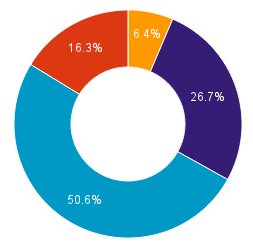
\includegraphics[width=\textwidth]{chart_2}
                \caption{Joren}
        \end{subfigure}%
        \begin{subfigure}[hb]{0.20\textwidth}
                \centering
                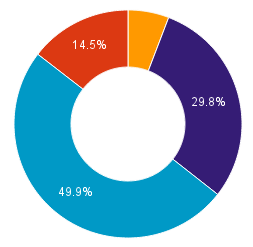
\includegraphics[width=\textwidth]{chart_3}
                \caption{Toon}
        \end{subfigure}%
        \begin{subfigure}[hb]{0.20\textwidth}
                \centering
                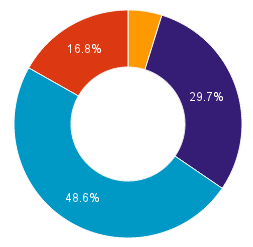
\includegraphics[width=\textwidth]{chart_4}
                \caption{Stef}
        \end{subfigure}%
        \begin{subfigure}[hb]{0.20\textwidth}
                \centering
                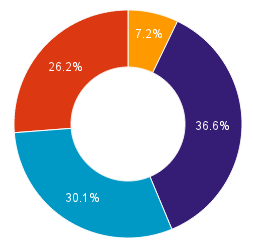
\includegraphics[width=\textwidth]{chart_5}
                \caption{Sophie}
        \end{subfigure}%
                \begin{subfigure}[hb]{0.20\textwidth}
                \centering
                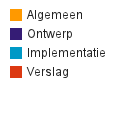
\includegraphics[width=\textwidth]{legende}
                \caption{Legend}
        \end{subfigure}%


 \caption{Overview of the division of tasks}
\label{fig:werkverdeling}
\end{figure}

%------------------------------------------------------ %
%														%
%           Glossary
%														%
%------------------------------------------------------ %
\section{Glossary}
\label{ssec:glossary}
\begin{description}
\item \gloss{ChangePolicyMenuAction}\\
\class{ChangePolicyManuAction} sets the policy in the menu for the \class{Launcher}

\item \gloss{ConsoleMenu}\\
\class{ConsoleMenu} is responisble for the menu items in the consoleView

\item \gloss{ConsoleMenuAction}\\
\class{ConsoleMenuAction} handles the actions in the menu of the consoleView

\item \gloss{ConsoleView}\\
\class{ConsoleView} is the console interface for the system

\item \gloss{Daemon} \\
\Daemon is responsible for executing the testruns. It can make use of different \class{Policy}'s to order the tests that need to be run.

\item \gloss{JUnit} \\
\junit is a unit testing platform

\item \gloss{Launcher} \\
The \class{Launcher} will launch the \Daemon .

\item \gloss{Policy} \\
A \class{Policy} imposes an order or filtering 

\item \gloss{RunListener} \\
Junit provides support for adding listeners while executing the testcases via \class{RunListener}. 

\item \gloss{RunNotifier} \\
A \class{RunNotifier} is a class, by which test fire events in the testrun flow.
Parties that are interested in these events can register a \class{RunListener} with this \class{RunNotifier}, so that they will be notified.

\item \gloss{TestRun}\\
\class{TestRun} is a testrun.

\item \gloss{TestRunCreator}\\
\class{TestRunCreator} creates testruns with different policies.

\end{description}
 

\end{document}